\chapter{Documentation tools}

Analysis of existing tools and user needs must precede project planning and development. This chapter attempts to answer these two questions:
\begin{enumerate}
    \item What is available?
    \item What do users want?
\end{enumerate}

\section{What is available?} \label{sec:whatisavailable}
The current documentation tool market provides the following solutions:

\begin{enumerate}
    \item DocFX\footnote{\nolinkurl{https://github.com/dotnet/docfx}{https://github.com/dotnet/docfx}}
    \item Doxygen\footnote{\nolinkurl{https://www.doxygen.nl/}{https://www.doxygen.nl/}}
    \item Source Browser\footnote{\nolinkurl{https://github.com/KirillOsenkov/SourceBrowser}{https://github.com/KirillOsenkov/SourceBrowser}}
    \item Vsxmd\footnote{\nolinkurl{https://github.com/lijunle/Vsxmd}{https://github.com/lijunle/Vsxmd}}
    \item vsdoc-2-md\footnote{\nolinkurl{https://github.com/discosultan/vsdoc-2-md}{https://github.com/discosultan/vsdoc-2-md}}
\end{enumerate}

What follows are evaluations of each tool that provides prospects on features and improvements the custom tool utilize.

\subsection{DocFX} \label{ssec:docfx}

\textit{DocFX} is an open-source documentation generation tool developed by Microsoft that supports \ref{gloss:dotnetlabel} languages, Java, JavaScript, TypeScript, Python, and others. Additionally, it can use raw \ref{gloss:markdown} files as input.

However, \textit{DocFX} only outputs static \ref{itm:html} pages. Therefore, the only available customizability is via templates for said static pages.

The tool is capable and is the go-to solution for \ref{gloss:dotnetlabel} projects, but it does not solve the task of outputting \ref{gloss:markdown} files.

Configuring and running \textit{DocFX} is unintuitive, as it provide no \ref{itm:gui}. Instead, it uses a configuration file. Moreover, the documentation for the tool leaves much to be desired, as it does not describe all possible settings.

\subsection{Doxygen} \label{sec:doxygen}

\textit{Doxygen} is the industry-standard documentation-generating tool originally made for C/C++ source code documentation. Support for popular programming languages, such as C\#, Java, Python, and many more, was added later.

The tool provides an extensive set of supported output formats:
\begin{itemize}
    \item Static \ref{itm:html}.
    \item \LaTeX\footnote{Document preparation system}.
    \item Man pages\footnote{User manual type that is part of Unix operating systems \cite{credocs_limited_latex_2022}}.
    \item \ref{itm:rtf}.
    \item \ref{itm:xml}.
\end{itemize}

It is possible to extend the tool, as it is open-source and available on GitHub. Unfortunately for \ref{gloss:dotnetlabel} developers, \textit{Doxygen} is written in C++, and its documentation does not provide clear guidelines for extending its support for output formats. Naturally, a curious programmer can deduce how to do that from the source code; however, this involves investing considerable time and effort.

Thankfully, configuring and executing \textit{Doxygen} is made simple with its \ref{itm:gui}.

\subsection{Source Browser}

\textit{Source Browser} is a tool that generates a website for browsing source code and its documentation. The tool is used by Microsoft, for example, to allow developers to browse the source code of \ref{gloss:dotnetlabel}.

The generated output is not entirely static and has to be hosted on an \ref{gloss:aspnetcore} website to support searching.

\subsection{Vsxmd} \label{ssec:vsxmd}

\textit{Vsxmd} generates a single \ref{gloss:markdown} file for all types in a given assembly. Moreover, the tool has no \ref{itm:ui} and works as a \ref{gloss:nuget} package that the project designated for documentation generation references. Thus, configuring this tool is done via \ref{gloss:dotnetlabel} project settings.

It is impossible to navigate the documentation as the tool does not generate links.

\subsection{Vsdoc-2-md}

\textit{Vsdoc-2-md} is an entirely unusable tool, as it is purely web-based and generates documentation from the provided \ref{itm:xml} documentation source file. The tool is limited to processing only one file at a time.

Just like \textit{\nameref{ssec:vsxmd}}, this tool does not generate links; thus, navigating the documentation is impossible.

\newpage

\section{What do users want?} \label{sec:whatdouserswant}
Surveying potential tool users is necessary to ensure that the developed product is utilized by more than its developer.
Thus, creating a questionnaire was the first step to success. Its purpose was to figure out the following key points:
\begin{itemize}
    \item Whether users already use documentation generation tools, and if so, which ones?
    \item What do users feel is missing from the tools they use?
    \item What do users believe should be carried over to the new tool from the ones they use?
    \item Whether users would integrate such tools into their \ref{itm:cicd} pipelines?
    \item What output formats do users want?
    \item What operating systems do users want the tool to work on?
    \item Would users find a \ref{itm:gui} beneficial for such a tool?
    \item Would users appreciate the tool being extensible via plugins?
    \item Would users be interested in contributing to the project?
\end{itemize}

\subsection{Questionnaire results}

What follows are the responses of the 22 participants of the questionnaire.

\subsubsection*{What output formats do you wish to have for your documentation?}

\begin{figure}[H]
    \centering
    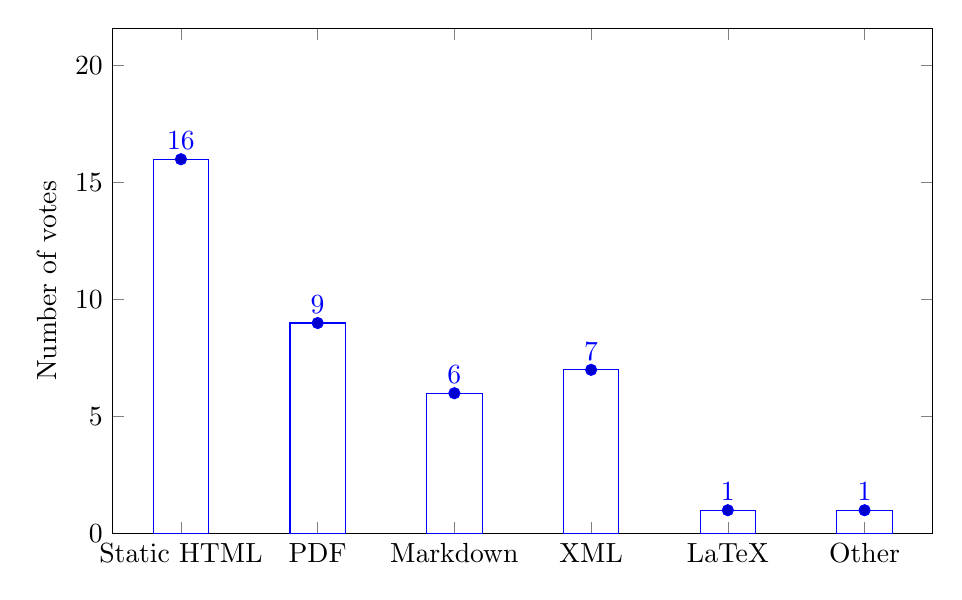
\begin{tikzpicture}
        \begin{axis}[
            symbolic x coords={Static HTML, PDF, Markdown, XML, LaTeX, Other},
            xtick=data,
            width=12cm,
            height=8cm,
            ymin=0,
            ymax=18,
            bar width=20pt,
            ylabel={Number of votes},
            enlarge y limits={value=0.2,upper},
            legend pos=north west,
            nodes near coords
        ]
            \addplot+[ybar] coordinates {
                (Static HTML,   16)
                (PDF,            9)
                (Markdown,       6)
                (XML,            7)
                (LaTeX,         1)
                (Other,          1)
            };
        \end{axis}
    \end{tikzpicture}
    \caption{What output formats do you wish to have for your documentation?}
    \label{fig:qOutputFormats}
\end{figure}

\textit{Other responses:}
\begin{itemize}
    \item AsciiDoc.
\end{itemize}

\subsubsection*{Would you integrate such a tool in your CI/CD process?}

\begin{figure}[H]
    \centering
    \begin{tikzpicture}
        \pie[sum=auto , after number=]{9/Yes, 2/No, 11/Maybe}
    \end{tikzpicture}
    \caption{Would you integrate such a tool in your CI/CD process?}
\end{figure}

\subsubsection*{How crucial is it for the tool to support these platforms?}

\begin{figure}[H]
    \centering
    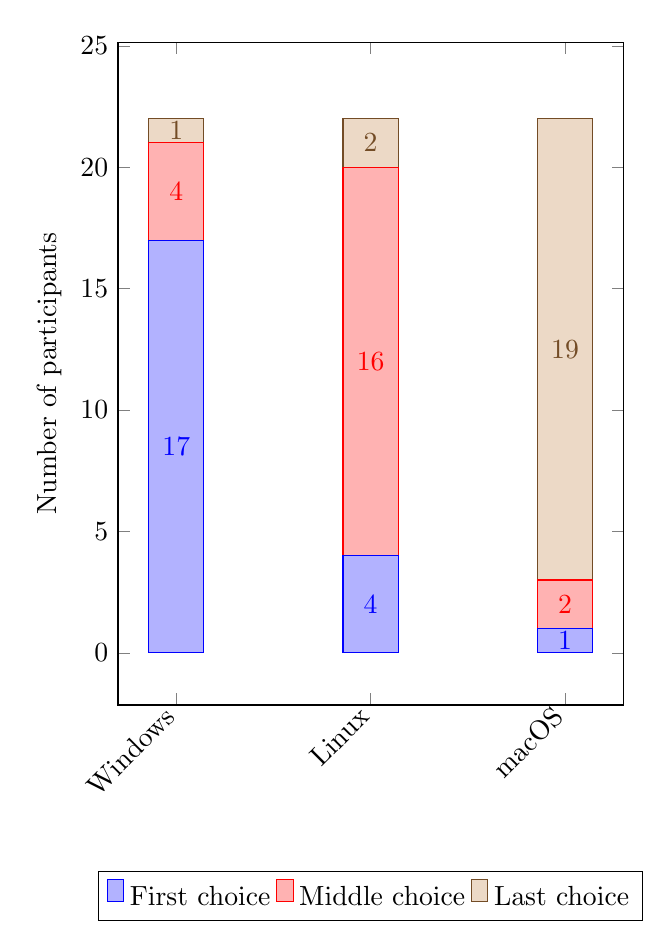
\begin{tikzpicture}
        \begin{axis}[
            ybar stacked,
            bar width=20pt,
            height=10cm,
            width=8cm,
            nodes near coords,
            enlargelimits=0.15,
            legend style={at={(0.5,-0.25)},
            anchor=north,legend columns=-1},
            ylabel={Number of participants},
            symbolic x coords={Windows, Linux, macOS},
            xtick=data,
            x tick label style={rotate=45,anchor=east},
            ]
        \addplot+[ybar] plot coordinates {(Windows,17) (Linux,4) (macOS,1)};
        \addplot+[ybar] plot coordinates {(Windows,4) (Linux,16) (macOS,2)};
        \addplot+[ybar] plot coordinates {(Windows,1) (Linux,2) (macOS,19)};
        \legend{\strut First choice, \strut Middle choice, \strut Last choice}
        \end{axis}
    \end{tikzpicture}
    \caption{How crucial is it for the tool to support these platforms?}
\end{figure}

\subsubsection*{Would it be beneficial to have a GUI instead of only a console?}

\begin{figure}[H]
    \centering
    \begin{tikzpicture}
        \pie[sum=auto , after number=]{12/Yes, 9/No, 1/Other}
    \end{tikzpicture}
    \caption{Would it be beneficial to have a GUI instead of only a console?}
\end{figure}

\textit{Other responses:}
\begin{itemize}
    \item I don't want separate docs, readable code is better.
\end{itemize}

\subsubsection*{Would you appreciate the tool being extensible via plugins?}

\begin{figure}[H]
    \centering
    \begin{tikzpicture}
        \pie[sum=auto , after number=]{17/Yes, 5/No}
    \end{tikzpicture}
    \caption{Would you appreciate the tool being extensible via plugins?}
\end{figure}

\subsubsection*{Are you using tools for documentation generation?}

\begin{figure}[H]
    \centering
    \begin{tikzpicture}
        \pie[sum=auto , after number=]{8/Yes, 14/No}
    \end{tikzpicture}
    \caption{Are you using tools for documentation generation?}
    \label{fig:qUsingToolsForDocGen}
\end{figure}

\subsubsection*{What documentation generating tools do you use?}

\begin{figure}[H]
    \centering
    \begin{tikzpicture}
        \pie[sum=auto , after number=]{3/DocFX, 2/Doxygen, 1/Slate, 1/Hugo}
    \end{tikzpicture}
    \caption{What documentation generating tools do you use?}
\end{figure}

\subsubsection*{What features from those tools you'd like to see in the resulting project?}

\textit{Responses:}
\begin{itemize}
    \item \ref{itm:gui} for less technical people.
    \item Links to external \ref{gloss:dotnetlabel} type references.
    \item Easy templating.
    \item Extended \ref{gloss:markdown} - custom short codes.
    \item Fast build speed for \ref{itm:cicd}.
    \item A capable \ref{itm:cli}.
    \item Class structures.
\end{itemize}

\subsubsection*{What features are missing in your current tool and would make you consider using the resulting project if they were to be provided by it?}

\textit{Responses:}
\begin{itemize}
    \item Better support for diagrams (like mermaid.js).
    \item A tool that could build a static site with a) editorial (\ref{gloss:markdown}) content b) \ref{gloss:dotnetlabel} \ref{itm:api} reference c) RESTful API documentation from \ref{gloss:aspnetcore} projects and/or OpenAPI definitions all under one umbrella.
\end{itemize}

\subsubsection*{Would you be interested in contributing to this project?}

\begin{figure}[H]
    \centering
    \begin{tikzpicture}
        \pie[sum=auto , after number=]{14/No, 6/Maybe}
    \end{tikzpicture}
    \caption{Would you be interested in contributing to this project?}
\end{figure}

\subsection{Questionnaire evaluation} \label{ssec:questionnaireeval}

Those who find a use for such tools want to export static \ref{itm:html} and to have the ability to extend the functionality via plugins.
Other responses displayed a clear division of needs regarding \ref{itm:cicd} integration, the target \ref{itm:os}, and the need for a \ref{itm:gui}.
The dominant documentation-generating tool for \ref{gloss:dotnetlabel} is \nameref{ssec:docfx} (see \ref{ssec:docfx}).

Questionnaire takeaways:

\begin{itemize}
    \item The majority neglects the importance of documenting code; thus, those who do and use documentation-generating tools are part of a minute subset of all developers (see figure \ref{fig:qUsingToolsForDocGen}).
    \item The tool should be cross-platform.
    \item The tool must have good performance.
    \item A console will be used by administrators of \ref{itm:cicd} pipelines and power users, while the \ref{itm:gui} will be for the rest.
    \item Support for \ref{itm:cicd} is to automate documentation generation fully.
    \item Even though the majority seeks to export to static \ref{itm:html} pages (see figure \ref{fig:qOutputFormats}), the project will focus on \ref{gloss:markdown} to fill  the market gap. The rest of the mentioned output formats will receive support later (see below).
    \item \textbf{Extensibility via plugins will be the key selling point of the tool - it will enable anybody to modify the functionality to meet their specific needs}.
    \item Future support for \nameref{ssec:docfx} (see \ref{ssec:docfx}) templates will help users migrate from said platform.
\end{itemize}